\section{Scheduling with Known Arrival Types: The WAIT Algorithm}
\label{sec:wait}

In this section, as a warm-up, we introduce the \textit{Waiting for Accumulated Inference Threshold} (WAIT) algorithm, a scheduling policy designed to maximize throughput in LLM inference systems under known prompt arrival types, while adhering to memory constraints and performance metrics including latency and time-to-first-token (TTFT). Leveraging the fluid dynamics established in Section \ref{sec:fluid}, our WAIT tries optimizes batch formation and scheduling by accumulating prompts until specific thresholds are met, ensuring efficient resource utilization in stochastic environments. We assume that the memory capacity $C\ge M^*,$ the equilibrium memory capacity given in \eqref{eq:memory_multi2} (otherwise the throughput can never approach the optimal fluid throughput \eqref{throughput_fluid_multiple} by Proposition \ref{prop::online policy expected throughput upper bound, multiple type}).

\subsection{Algorithm Overview}
The WAIT algorithm operates by maintaining $m$ inventories of prompts and tracking their current inventory across all types and stages until the system reaches a state in accordance with the fluid dynamics. For each prompt type \( j \in [m] \) and stage \( k \in \{0, 1, \dots, l_j'\} \), the algorithm sets a threshold \( n_j \) for type \( j \) prompts, where \( n_j \) is derived from the fluid dynamics presented in Section \ref{sec:fluid} and will be detailed subsequently.

At each continuous time \( t \), the WAIT algorithm monitors the current inventory \( n_{jk}^t \), defined as the number of waiting prompts of type \( j \) at stage \( k \), for \( k = 0, 1, \dots, l_j' \), alongside stochastic arrivals following Poisson distribution $\text{Poisson}(\lambda_j)$ in each unit time interval. At time \( t \), the algorithm incorporates type \( j \) prompts into the batch for a new iteration whenever the inventory level satisfies:
\[
n_{j0}^t \geq n_j.
\]
This condition implies that type \( j \) prompts are processed at time \( t \) only if the number of type \( j \) prompts awaiting prefill is at least \( n_j \). When this criterion is met, WAIT constructs a batch \( B^t \) by selecting \( \min\{n_j, n_{jk}^t\} \) prompts of type \( j \) at each stage \( k = 0, 1, \dots, l_j' \) for all \( j \) that satisfy the threshold condition. This batch is then processed in the current iteration, utilizing GPU memory proportional to the total number of tokens processed. Following processing, the inventory is updated, and prompts progress to their subsequent stages as appropriate. If the condition is not satisfied for any \( j \), the algorithm pauses, permitting additional prompts to accumulate in the next time step. Moreover, the algorithm preserves the KV caches computed for waiting prompts throughout this process, thereby avoiding redundant computations. This threshold-based strategy ensures that the batch composition aligns with the fluid dynamics, striving to minimize memory waste and enhance throughput in heavy-traffic scenarios, which will be elaborated later. The complete specification of the WAIT algorithm is presented in Algorithm \ref{alg:wait}. Figure \ref{fig:wait} shows how WAIT works at batching.
\begin{figure}
    \centering
    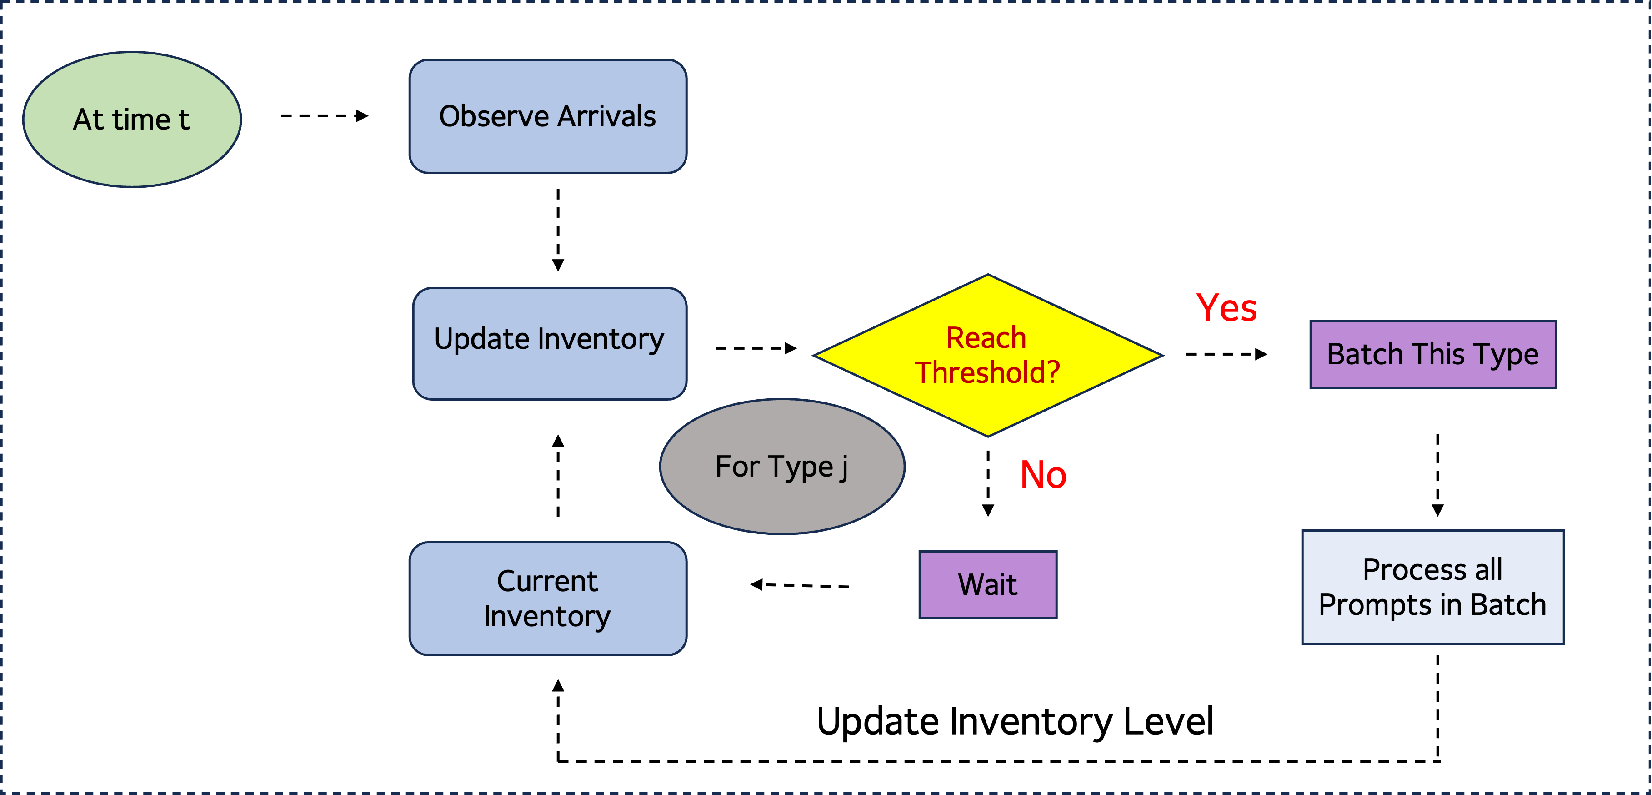
\includegraphics[width=0.9\linewidth]{Experiments_pdf/fig_WAIT.pdf}
    \caption{Pipeline of Algorithm \ref{alg:wait}}
    \label{fig:wait}
\end{figure}

\begin{algorithm}[h]
\caption{WAIT: Waiting for Accumulated Inference Threshold}
\label{alg:wait}
{\small\linespread{1.0}\selectfont
\begin{algorithmic}[1]
\Require Memory $C$, arrival rates $\lambda_j$, thresholds $n_j$ satisfying \eqref{eq:wait_thresholds}, $\forall j \in [m]$
\State Initialize prompt inventory $n_{jk} \gets 0$ for all $j \in [m], k \in \{0, 1, \dots, l_j'\}$ 
\State Initialize event queue with arrival events for each type $j$
\State Set current time $t \gets 0$  
\While{True}
    \State Wait for the next event (arrival or batch completion) 
    \If{event is an arrival of type $j$}
        \State Update inventory: $n_{j0} \gets n_{j0} + 1$  \Comment{Add new prompt to waiting queue of prefill phase}
        % \State Schedule next arrival for type $j$ based on $\text{Exponential}(\lambda_j)$  \Comment{Generate time for next arrival}
    \ElsIf{event is a batch completion}
        \State Update inventory: For each $j$ in batch $B$, $n_{jk} \gets n_{jk} - \min\{n_j, n_{jk}\}$ for $k = 0, \dots, l_j'$  
        % \Comment{Remove processed prompts}
        \State Advance prompts: For each $j$, move $\min\{n_j, n_{jk}\}$ prompts from stage $k$ to $k+1$  
        % \Comment{Progress to next stage}
        \State Clear KV caches for prompts reaching stage $l_j' + 1$  \Comment{Free memory for completed prompts}
    \EndIf
    \State Check if $n_{j0} \geq n_j$ for any $j \in [m]$  \Comment{Check threshold for batching}
    \If{condition $n_{j0} \geq n_j$ is met for some $j$}
        \State Form batch $B$ by selecting $\min\{n_j, n_{jk}\}$ prompts of type $j$ at each stage $k$ for all $j$ meeting the condition  \Comment{Create batch}
        % \State Compute processing time $\tau$ based on batch size (e.g., total tokens)  \Comment{Determine processing duration}
        \State Process batch $B$, keep prompts outside the batch waiting and donot delete their KV caches
        % \Comment{Start processing, }
        % \State Batch completion event at time $t + \tau$  
        % \Comment{Set event for batch finish}
    \EndIf
\EndWhile
\end{algorithmic}
}
\end{algorithm}
\subsection{Heavy Traffic Analysis}
\label{subsec:heavy_traffic}
We evaluate the performance of WAIT in heavy traffic scenarios, where the prompts arrive intensively. Specifically, we consider the \emph{conventional heavy traffic scaling} in standard queueing theory (see e.g. \cite{mandelbaum1998strong}), where arrival rates and processing speeds are scaled up. In this regime, we scale the arrival rates to $\lambda_j^{(\zeta)} = \zeta \lambda_j$ and processing speeds accordingly ($(d_0^{(\zeta)},d_1^{(\zeta)})=(\zeta^{-1}d_0,\zeta^{-1}d_1)$ while keeping memory capacity $C$ fixed. It can be also regarded as scaling the total time horizon $T$ to $\zeta T,$ while keeping the arrival rates and processing speed unchanged. The system experiences increased load as $\zeta \to \infty$, allowing us to study throughput stability under high demand.
% and (ii) the \emph{many-server heavy traffic scaling}, where both arrival rates and memory capacity are scaled proportionally.

% \textbf{Conventional Heavy Traffic:} 

% \textbf{Many-Server Heavy Traffic:} Here, we scale arrival rates to $\lambda_j^{(\zeta)} = \zeta \lambda_j$ and memory capacity to $C^{(\zeta)} = \zeta C$, compressing the time horizon by a factor of $1/\zeta$ (i.e., observing over $[T]$). This regime examines system performance when both demand and resources grow proportionally.

\textbf{Performance Metric:} We focus on the average throughput, denoted $\throughput^{(\zeta, \pi)}$, where $\pi$ represents the WAIT policy, defined as:
\[
\throughput^{(\zeta, \pi)} = \frac{1}{\zeta T} \sum_{j=1}^m N_j^{(\zeta, \pi)},
\]
with $N_j^{(\zeta, \pi)}$ being the total number of type-$j$ tokens processed under scaling $\zeta$. The average latency $\Latency^{(\zeta,\pi)},\TTFT^{(\zeta,\pi)}$ and TTFT are defined similarly by dividing the quantity by $\zeta$. Our objective is to demonstrate that $\throughput^{(\zeta, \pi)}$ approaches the fluid equilibrium benchmark $\throughput^* = \sum_{j=1}^m (1+ l_j') \lambda_j$ (\ref{throughput_fluid_multiple}) as $\zeta \to \infty$ while giving bound to the latency and TTFT.

\subsection{Theoretical Analysis}
\label{subsec:main_theorem}
When the memory constraint satisfies \(C \geq M^*\), consider the WAIT policy \(\pi\), parameterized by \([n_1, \dots, n_m]\), where \(n_j\) represents the threshold for the number of type \(j\) prompts at each stage. We will demonstrate that the WAIT policy is asymptotically optimal when the thresholds meet the following inequalities:
\begin{equation}
\label{eq:wait_thresholds}
\begin{aligned}
\Delta T(n_{1:m}) &:= d_0 + d_1 M^{\pi} \leq \tfrac{n_j}{\lambda_j},\, \forall j\in[m],\\
 M^{\pi} &= \sum_{j=1}^m n_j (l_j' + 1) \big(l_j + \tfrac{l_j'}{2}\big)
\end{aligned}
\end{equation}
where \(M^*\) is defined in Equation \eqref{eq:memory_multi2}. To understand the intuition, one can refer to a derivation similar to that in Equation \eqref{eq:time_fluid} and note that, if type \(j\) is included in the current iteration, the expected number of arrivals of type \(j\) during this iteration will not exceed \(n_j\). This indicates that the system’s behavior closely approaches the fluid equilibrium. Formally, our main theorem is presented below.

% we obtain the policy class $\Pi$, each $\pi = [n_1,\cdots,n_m]\in \Pi$ with corresponding memory capacity $M^{\pi} \geq  M^*$.

% $\forall \pi \in \Pi$, when prompts of all $m$ types are in the same batch, $\text{Arrival}_j\leq \text{Completion}_j$. Indeed, when type $j$ is in the batch, no matter what the other types are in the batch, we have that $\text{Arrival}_j\leq \text{Completion}_j$. Specifically, when $M^c = M$, the policy is $\pi = [ \frac{n_1^*}{l_1^\prime+1},\,\cdots,\,\frac{n_m^*}{l_m^\prime+1} ]$. 

% The following theorem establishes the near-optimality of WAIT under heavy traffic conditions.
\begin{theorem}
\label{thm:wait_heavy_traffic}
    Assume the thresholds $\pi=[n_1,\dots,n_m]$ satisfy \eqref{eq:wait_thresholds}, then we have 
% \begin{equation*}
%     \begin{aligned}
%         &\throughput^*-\ex{}{\throughput^{(\zeta,\pi)}}=O((\zeta T)^{-\frac{1}{2}}),\\ 
% &\ex{}{\Latency^{(\zeta,\pi)}}=O\prn{(\zeta T)^{\frac{1}{2}}},\\
% &\ex{}{\TTFT^{(\zeta,\pi)}}=O\prn{(\zeta T)^{\frac{1}{2}}}.
%     \end{aligned}
% \end{equation*}
$$
\begin{aligned}
    &\throughput^*-\ex{}{\throughput^{(\zeta,\pi)}}=O((\zeta T)^{-\frac{1}{2}}),\\ 
&\ex{}{\Latency^{(\zeta,\pi)}},\,\ex{}{\TTFT^{(\zeta,\pi)}}=O\prn{(\zeta T)^{\frac{1}{2}}}.
\end{aligned}
$$
    Moreover, when we have $\Delta T_{[1,\dots,m]}<n_j/\lambda_j,\forall j\in[m]$ where $\Delta T_{[1,\dots,m]}$ is defined in \eqref{eq:wait_thresholds}, it holds that
$$    \begin{aligned}
        &\throughput^* - \ex{}{\throughput^{(\zeta,\pi)}} = O(1/(\zeta T)), \\ 
&\ex{}{\Latency^{(\zeta,\pi)}},\, \ex{}{\TTFT^{(\zeta,\pi)}} = O(1).
    \end{aligned}$$
\end{theorem}



% \begin{theorem}
% \label{thm:wait_heavy_traffic}
% Under the conventional heavy traffic regimes, the WAIT algorithm achieves near-optimal throughput. Specifically:
% % \begin{itemize}
% %     \item In the many-server heavy traffic regime:
% %     \[
% %     \liminf_{\zeta \to \infty} \zeta^{-1} \mathbb{E} \left[ \throughput^{\zeta, \pi} \right] \geq (1 - T^{-1}) \throughput^*,
% %     \]
% %     where the time horizon is $T$.
% % \end{itemize}
% when $C = M^*$, we have that $\pi = [\frac{n_1^*}{l_1^\prime+1},\,\cdots,\, \frac{n_m^*}{l_m^\prime+1}]$. This is a special case where all types satisfy the condition $\Delta T_{[1,\cdots,m]} = \frac{n_j}{\lambda_j}$. So with the union bound, we have the expected upper bound of the throughput gap to the $\text{Throughput}^*$ under the fluid system \gan{ref, and the prop~\ref{prop::online policy expected throughput upper bound, multiple type} shows that this is the upper bound}.
% $$\frac{1}{S}\sum_{j=1}^m \ex{}{W_S^{(j)}}\leq \frac{1}{S}\sum_{j=1}^m \lambda_j +\sum_{j=1}^m \sqrt{\frac{1}{S}\lambda_j} $$
% In \textbf{Conventional Heavy-Traffic} case,
% $$\frac{1}{S^{\zeta }}\sum_{j=1}^m \lambda_j^{\zeta } +\sum_{j=1}^m \sqrt{\frac{1}{S^{\zeta }}\lambda_j^{\zeta }}  =\frac{1}{\zeta S}\sum_{j=1}^m \lambda_j +\sum_{j=1}^m \sqrt{\frac{1}{\zeta S}\lambda_j} \to 0, \,\zeta \to \infty.$$
% With the expected end-to-end latency
% $$\frac{1}{S}\cdot\Delta T_{[1,\cdots,m]} \cdot \left(\sum_{j=1}^m \lambda_j +\sum_{j=1}^m \sqrt{\lambda_j\cdot S} \right) \sim \Omega(\sqrt{\frac{1}{S}})$$

% When all $m$ types satisfy the condition $\Delta T_{[1,\cdots,m]} < \frac{n_j}{\lambda_j}$, the expected upper bound of the throughput gap is bounded:
% $$\frac{1}{S}\sum_{j=1}^m \ex{}{W_S^{(j)}}\leq \frac{1}{S}  \sum_{j=1}^m \left(2n_j+ \frac{\lambda_j \cdot \Delta T_{[1,\cdots,m]}}{2\cdot\left(n_j - \lambda_j\cdot \Delta T_{[1,\cdots,m]}\right)}\right) $$
% with the bounded expected end-to-end latency
% $$ \Delta T_{[1,\cdots,m]} \cdot\frac{1}{S}\sum_{j=1}^m \ex{}{W_S^{(j)}}\leq \Delta T_{[1,\cdots,m]} \cdot\frac{1}{S} \sum_{j=1}^m \left(2n_j+ \frac{\lambda_j \cdot \Delta T_{[1,\cdots,m]}}{2\cdot\left(n_j - \lambda_j\cdot \Delta T_{[1,\cdots,m]}\right)}\right) \sim \Omega (\frac{1}{S})$$
% \end{theorem}
The proof employs the coupling technique from queueing theory. We construct a stochastic process that shares the same arrival pattern as the original system but features processing times that are at least as long as those observed in the actual dynamics of the WAIT algorithm at each iteration. We establish that this constructed stochastic process dominates the real dynamics, thus yielding an upper bound on the performance gap of our algorithm. Our heavy-traffic analysis reveals that the WAIT algorithm achieves near-optimal throughput relative to the fluid optimal benchmark. Detailed proofs are available in Appendix \ref{appexidx::proof of wait_heavy_traffic}.

It is noteworthy that the results concerning different performance metrics in Theorem \ref{thm:wait_heavy_traffic} matche the worst-case lower bounds for latency and Time to First Token (TTFT). See the following proposition.
\begin{proposition}\label{prop::simple random walk, tight bound}
There exists an instance where \( C = M^* \), and for any non-predictive online policy \(\pi\), the expected average latency and TTFT satisfy
\[
\mathbb{E}[\Latency^{(\zeta,\pi)}],\quad \mathbb{E}[\TTFT^{(\zeta,\pi)}] = \Omega((\zeta T)^{1/2}).
\]
\end{proposition}
Moreover, we demonstrate that the latency for type \( j \) prompts depends exclusively on the relationship between \(\Delta T_{[1,\dots,m]}\) and $n_j/\lambda_j$. Specifically, when \(\Delta T_{[1,\dots,m]} < n_j/\lambda_j\), the average latency and TTFT for type \( j \) prompts are \( O(1) \), offering a more precise performance estimate than that provided in Theorem \ref{thm:wait_heavy_traffic}. A detailed discussion is presented in Appendix \ref{appexidx::proof of wait_heavy_traffic}.

Another interesting result is that, the First-Come-First-Serve (FCFS) policy, which processes arriving prompts in the order of their arrival as long as memory permits, will have poor theoretic performance. See the proposition below.
\begin{proposition}\label{prop:lower_bound_FCFS}
When the memory capacity \(C\) equals the equilibrium memory \(M_j^*\), there exists an instance where the First-Come-First-Serve (FCFS) policy described above incurs a throughput gap of \(\throughput^* - \mathbb{E}[\throughput^T] = \Omega(1)\) as \(T \to \infty\).
\end{proposition}
By Proposition \ref{prop:lower_bound_FCFS}, when the memory capacity equals the equilibrium memory \(M_j^*\), we can see that the FCFS can never reach asymptotically optimal performance. Indeed, this myopic policy may have to frequently remove ongoing prompts to accommodate new arrivals and require those preempted prompts to restart subsequently, which yields its sub-optimal performance in throughput. Detailed proofs are presented in Appendix \ref{appendix::proof of lower bound of of FCFS}.

% 1. When $ \Delta T_{[1,\cdots,m]} = \frac{n_j}{\lambda_j}$, we have that
% $$\lambda_j\cdot \Delta T = n_j\Rightarrow \ex{}{Y_s^{(j)}}=0.$$
% So by Lemma~\ref{lemma::throughput gap}, we have that
% $$\ex{}{W_S^{(j)}}\leq \ex{}{\tilde{W}_S^{(j)}}\leq \lambda_j + \sqrt{\lambda_j S}$$

% \gan{and the Proposition~\ref{prop::simple random walk, tight bound} of simple random walk shows that the bound is tight.}

% 2. When $\Delta T_{[1,\cdots,m]} < \frac{n_j}{\lambda_j}$, the expectation $\ex{}{Y_s^{(j)}}<0$. The coupled process $\tilde{W}_s^{(j)}$ has a negative drift. Since
% \begin{align*}
% \text{Var}(Y_s^{(j)} )&= \text{Var}(X_s^{(j)} )  = \lambda_j \cdot \Delta T_{[1,\cdots,m]}\\
% \left| \ex{}{Y_s^{(j)}} \right| &= n_j - \lambda_j\cdot \Delta T_{[1,\cdots,m]}
% \end{align*}
% By Kingman, we have that
% $$\ex{}{W_S^{(j)}}\leq \ex{}{\tilde{W}_S^{(j)}}\leq 2n_j + \frac{\text{Var}(Y_s^{(j)} )}{2\left| \ex{}{Y_s^{(j)}} \right| } =2n_j+ \frac{\lambda_j \cdot \Delta T_{[1,\cdots,m]}}{2\cdot\left(n_j - \lambda_j\cdot \Delta T_{[1,\cdots,m]}\right)}$$

% \textbf{Proof Sketch:} The proof analyzes the queue dynamics under WAIT. By construction, WAIT processes batches only when inventory levels $n_{jk}^t$ meet or exceed the thresholds $n_{jk}^*$, aligning with the fluid equilibrium. For the many-server regime, scaling $\lambda_j$ and $C$ by $\zeta$ ensures resource availability grows with demand, but finite horizon $T$ introduces a boundary effect of order $T^{-1}$. In the conventional regime, the extended horizon $\zeta T$ allows throughput to stabilize at $\throughput^*$ as waiting times diminish relative to the timescale. Using renewal theory and Poisson process properties, we bound the expected waiting times (Lemmas~\ref{throughput gap}--\ref{lemma::throughput gap}) and show convergence to the fluid benchmark. The detailed proof is relegated to Appendix~\ref{app:proof_wait}.

% \subsection{Discussion}
% \label{subsec:wait_discussion}

% Our WAIT algorithm provides a scheduling mechanism for LLM inference by aligning batch 
%  with the fluid model's optimal solution. Its threshold-based strategy mitigates inefficient and overloaded batching, particularly under high demand where memory and processing resources are constrained. The heavy traffic analysis shows that WAIT achieves near-optimal throughput compared with the fluid optimal benchmark. Detailed proofs are provided in Appendix~\ref{appexidx::proof of wait_heavy_traffic}.



A limitation of WAIT is its reliance on known arrival types and rates, which may not hold in realistic environments (though we can approximate it by using predictors, see e.g. \citep{fu2024efficient}). In the next section, we address this issue by extending WAIT to handle unknown arrival types, introducing a nested variant that adapts to stochastic settings with unknown prompt types upon arrival.